\documentclass[senior]{IPSstyle}

  \Year{2018}
  \Month{July}
  \Author{44161643-2: HOU BOWEI}

  \Title{Without Wearing Device Gaze Estimation from Image}

  \Advisor{Professor Yoshie}

\usepackage{amssymb,amsmath}

\usepackage{mathptmx}
\usepackage{helvet}
\usepackage{courier}
\usepackage{type1cm}

\usepackage{makeidx}
\usepackage{graphicx,subfigure}
\usepackage{multicol}
\usepackage{multirow}
\usepackage[bottom]{footmisc}

\usepackage{mathrsfs}
\usepackage{amssymb,amsmath}
\usepackage{amsfonts}
\usepackage{color}
\usepackage{CJKutf8}

\usepackage{listings}
\usepackage{algorithm,algorithmicx,algpseudocode}
\usepackage[toc,page,title,titletoc,header]{appendix}

\renewcommand{\algorithmicrequire}{\textbf{Input:}}
\renewcommand{\algorithmicensure}{\textbf{Output:}}

\Abstract{
Gaze estimation is a hot and traditional area in both computer vision and interaction. In the 90s, gaze estimation was developed by physics scientists, and the main usage is in the medicine surgery area. In that era, gaze estimation needs a lot of equipment on the head and a laboratory with lots of sensors. As the time moving on, the equipment is becoming smaller and the number of sensors are becoming lesser. However, we still need calibration device or eye-tracker facilities. 
Normally, a gaze estimation method is one kind of pipe line. They will use sensors to extract parameters of the environment. Such as illumination, position of the camera and the distance between the person and camera. After that, eye detector device is applied to take picture near your eyes and then get the shape of the eyeball. Finally, all the data extracted from the equipment, which as the landmarks of the head and eyes, will be fixed into a physical model of human’s head, with the predefined math equation eye direction can be calculated.
Here comes up a purpose, why don’t we use images only to detect the gaze direction. Inspired by the potential power of convolutional neural network which is proved to be good at extract information from image, it will be a convenient way to make an end-to-end algorithm based on specific neural network.
}

\Keywords{Convolutional Networks, Gaze Estimation, Deep Learning, Computer Vision, Eye Gaze}

\Acknowledgments{
I came to Japan almost two years ago without any experience of Japanese. Japan is new to me, but the Japanese are so nice that they make me feel at home. 

I really appreciate the first year learning lessons in IPS, teachers help me to base the fundamental knowledge of data science, like the NLP concerning class, Computer Vision concerning class digital signal processing, and machine learning concerned pattern recognition.

The laboratory is another place where I really admire to live in. Professor Yoshie helped us with supporting very powerful server to do experiments. Also we have a very comfortable enviorment in the lab. 

At last, I want to pay appreciation to my fellows, all the students in the lab. We study together and solve problems together, during the two-years learning process, not only knowledge but also friendship is developed. The memory of being together will reminds all my life long.
}


\begin{document}

 \makepreliminarypages
 \singlespace
 \frontmatter
 \tableofcontents
 \listoffigures
 \listoftables
 \mainmatter
 \clearemptydoublepage
 \setlength{\baselineskip}{23.0pt}

\chapter{Introduction} \label{introduction}
%%%%%%%%%%%%%%%%%%%%%%%%%%%%%%%%%%%%%%%%%%%%%%%%%%%%%%%%% Chapter Introduction
\section{Background}

Gaze estimation is a traditional area in computer vision and computer interaction. 
Since long time ago, finding the gaze direction is the object in medical and facial analyze projects. 
In the ancient times, such kind of technologies are based on heavy equipment, including electro-occulography and coil embed lens. 
When it comes to video eye gaze studying\cite{mohamed2007history}, the first one is concerned with airplane pilot, mainly for flight control systems in 1940s. 
After that the technology develops toward head mounted trackers, and in 1970s, in order to improve accuracy and reducing limitations. 
As the hardware had developed so fast, in 1980s, it is the first time when real-time eye gaze estimation can take place. 
But it is only constrained to medical and cognitive researches\cite{borji2013state}. 
The situation changed after 2000, researchers pay more attention to computer interaction applications.
Like the broadly used desktop computers and televisions, it happened in playing station, video analyzing and commercial web studying.
Although such area gained a lot of achievements, it is still a hot topic. The equipment used in such areas is becoming more handle and cheaper, we are still looking for some method to get rid of devices.

The main structure to predict eye gaze direction is using a step-by-step pipeline structure. 
In order to find out the transformation matrix from real world coordination to image coordination.
The first step is calculating homograph transformation matrix, and then use camera calibration model to extract features used for RANSAC algorithm.
From the pipeline the points in gaze direction in real world of a three dimensional vector can be transformed to two dimensional line in the image.

Convolutional networks begin in 2012 showed its power of understanding images. 
New structures in deep learning area with convolutional networks can detect object and recognize object.
Especially in complex problems, convolutional neural network can extract features in the image and then establish relationship with target labels by training with large amount of data.
This Idea have taken a impact in computer vision studies.
Researchers need to make their data and label them to feed into networks.
By the power of transfer learning, even unrelated networks studies trained by total different data can have a common sense of object recognition.


\subsection{Homograph}
%单应性变换
In order to reflect same object in one image's points into the other one. 
Homograph transformation should be used.
The reflection can be one image or one surface in the three dimensional coordinate.
It is practical to be applied in image registration, image correction and image texture distortion.
It is performed normally be a matrix multiplication by the homogeneous equation.
\[\begin{bmatrix} x'\\ y'\\ w' \end{bmatrix} = \begin{bmatrix} h_1 & h_2 & h_3\\ h_4 & h_5&h_6 \\ h_7 & h_8 & h_9 \end{bmatrix} \begin{bmatrix} x\\ y\\ w \end{bmatrix} \text{or } \bold{x'= Hx}\]

There are three kinds of algorithms for homograph, one is DLT(Direct Linear Transformation), second is Affine transformation, image distortion.
The different in such algorithms is about degree of freedom. 

\begin{figure}
    \centering
    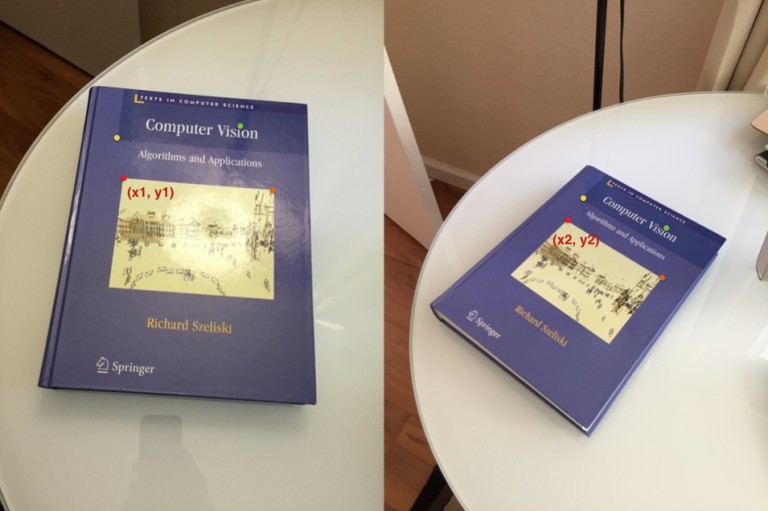
\includegraphics[width=15cm]{MasterThesis-master/homography_example.jpg}
    \caption{point (x1,y1) on the book on the left image is corresponded to point (x2, y2) in right one. the formulation can be calculated as 
    $x' = \begin{bmatrix} A & t \\ 0 & 1 \end{bmatrix} x$, $x'= \begin{bmatrix} x1 & y1 & w' \end{bmatrix}^{T}$, $x= \begin{bmatrix} x2 & y2 & w \end{bmatrix}^{T}$}
    \label{fig:homography example}
\end{figure}

As Fig. \ref{fig:homography example} shows the homography matrix is the key to match correspondent points in both pictures.
Usually traditional algorithm try to find out the matrix by using SVD\cite{essig2010fully}.


\subsection{3D Reprojection}
%%%%%%%%%%%%%%%%%%%%%%%%%%%%%%%%%%%%%%%%%%%%%%%%%%%%%%%%%%%%%%%%%%%%%%%%%%%%%%%

\section{Application Scenes}
\subsection{Special Device to Check Pupil}
\subsection{Car Industry Detect Eye Movement}
\subsection{Play Station}

%%%%%%%%%%%%%%%%%%%%%%%%%%%%%%%%%%%%%%%%%%%%%%%%%%%%%%%%%%%%%%%%%%%%%%%%%%%%%%%


\section{Organization of the thesis}

%%%%%%%%%%%%%%%%%%%%%%%%%%%%%%%%%%%%%%%%%%%%%%%%%%%%%%%%%%%%%%Chapter Related work
\chapter{Related Work} \label{related_work}
%%%%%%%%%%%%%%%%%%%%%%%%%%%%%%%%%%%%%%%%%%%%%%%%%%%%%%%%%%%%%%Chapter 3

%%%%%%%%%%%%%%%%%%%%%%%%%%%%%%%%%%%%%%%%%%%%%%%%%%%%%%%%%%%%%%%%%%%%%%%%%%%%%%%

\section{Traditional gaze estimation}
\subsection{Original Pipeline Algorithm}
\section{Deep learning based methods}
\subsection{Gaze Estimation in the Wild}
\subsection{Eye Tracking for Everyone}

%%%%%%%%%%%%%%%%%%%%%%%%%%%%%%%%%%%%%%%%%%%%%%%%%%%%%%%%%%%%%%%%%%%%%%%%%%%%%%%

\chapter{Methodology} \label{methodology}
%%%%%%%%%%%%%%%%%%%%%%%%%%%%%%%%%%%%%%%%%%%%%%%%%%%%%%%%%%%%%%%%%%%%%%%%%%%%%%%
\section{Network Structure} \label{network structure}
\subsection{Pre-trained Model}
\subsection{Transfer Learning}
\subsection{Attention Model}

\section{Training Phase} \label{training phase}
\subsection{Formulation of the input}
\subsection{Data Augment}
\subsection{Loss Function}


\section{Testing Phase} \label{testing phase}
\subsection{One Person Output}
\subsection{Different Person Output}
\subsection{Points Based Structure}

%%%%%%%%%%%%%%%%%%%%%%%%%%%%%%%%%%%%%%%%%%%%%%%%%%%%%%%%%%%%%%%%%%%%%%%%%%%%%%%
\chapter{Experiments} \label{experiments}
\section{Images in MPII}
\subsection{Sources}
\subsection{Methods to Record}
\section{Datasets Structure}
\section{Results Display}


\bibliographystyle{IEEEtran}
\bibliography{LUOreference}
\end{document}
